%\documentclass[11pt,xcolor=gray,handout]{beamer}
\documentclass[hyperref={pdfpagelabels=false}]{beamer}
\let\Tiny=\tiny
\mode<presentation>{
\usetheme{Singapore}
%\usecolortheme{beaver}
\usefonttheme{serif}
}
\usepackage{default}
\usepackage{verbatim}
%\usepackage{ucs}
\usepackage[utf8]{inputenc}
\usepackage{gb4e}
\usepackage[T1]{fontenc}
\usepackage{ tipa }
\usepackage{qtree}
\usepackage{synttree}
\usepackage{color}
\usepackage{tree-dvips}
\usepackage[absolute,overlay]{textpos}
%\usepackage{covington-beamer}
\usepackage{lmodern}
\usepackage{natbib}
\usepackage{graphicx}
\usepackage{booktabs}
%\usepackage{pdfpages}


%\usepackage{memoir}
%\usepackage{relsize}
%\newcommand{\subscript}[1]{\raisebox{-0.25em}{\smaller #1}}
%\logo{\includegraphics[height=0.5cm]{hilogo2.png}}
\setbeamertemplate{footline}[frame number] 
%gets rid of navigation symbols
\setbeamertemplate{navigation symbols}{}

%A Role for Early Life Androgens on Gendered Language Use

\title{Gender, language change, and hormonal organising effects}
\author{Joel C. Wallenberg and Josef Fruehwald\\Newcastle University, University of Edinburgh\\\texttt{joel.wallenberg@ncl.ac.uk\\ josef.frueh@ed.ac.uk}}
%\institute{Workshop on Language Variation and Change and Cultural Evolution}
%\date[]{ \\ York}

\begin{document}

\begin{frame}[plain]
\titlepage
\end{frame}


\section{Introduction}
\begin{frame}{Introduction}

	
	\begin{itemize}
		\item \textbf{Linguistic sex/gender effects:} it is well known that speaker-sex has a stochastic effect on the frequency with which linguistic variants are used. Reasons unknown.
		\item \textbf{Hormonal Organising Effects:} the action of sex steroids during sensitive period for sexual differentiation 
		(\textsl{in utero}, esp. weeks 8-24 for humans), affecting primary/secondary sex characteristics, and ``gender'':
			\begin{itemize}
				\item Behaviour: mating behaviours in mammals, sexuality and gender identity in humans, pair-bonding and other behaviours in birds.
				\item Brain morphology: e.g. the sexually-dimorphic nucleus of the pre-optic area in mammals, including humans, with a correlate in birds; also e.g. parts of the avian song system \citep[][]{balthazartetal2009}.
				\item Not to be confused with activational, or circulating hormone effects, which are often independent.
			\end{itemize}
	\end{itemize}
	
\end{frame}


\begin{frame}
\frametitle{Outline}
\tableofcontents
\end{frame}


\section{Linguistic Sex Effects}
\subsection{Reported Effects}

\begin{frame}{Sex/Gender and Change from Below}
\begin{itemize}
	\item When linguistic changes begin, a new linguistic feature is innovated, and has to spread through a population.
	\item As it spreads, there is both inter-speaker and intra-speaker variation, essentially for all variants studied.
	\begin{exe}
		\ex \begin{xlist}
			\ex Have you any money?
			\ex Do you have any money?
		\end{xlist}	  (British Isles)
		\ex John is going to his \{$[$haus$]$/$[$hæ\textschwa s$]$\}. \\(Philadelphia English)
		\ex I want to, \{\textsl{um, uh}\}, tell you some things. \\(All Englishes so far, and German and Dutch?!)
	\end{exe}
		
	\item Women tend to lead \textbf{changes from below} the level of consciousness (see \citealt[][Chapt. 8]{labov2001} long list of references up to that date).
\end{itemize}
\end{frame}

\begin{frame}{Sex and Change from Below, /aw/ \small{\citep{fruehwald2013} \\n_{speakers} = 308, n_{vowels} = 16046}}
	
		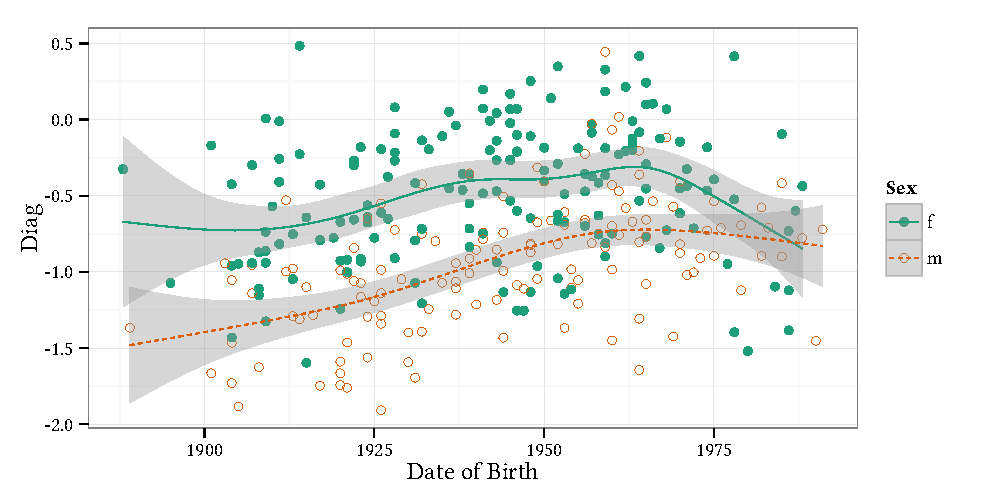
\includegraphics[width=1.15\textwidth]{figures/ch4awTrajectory.pdf}
		\begin{center}
		
	\end{center}
\end{frame}

\begin{frame}{Sex and Change from Below, /uw/ \small{\citep{fruehwald2013}\\ n_{speakers} = 308, n_{vowels} = 16232}}
	
		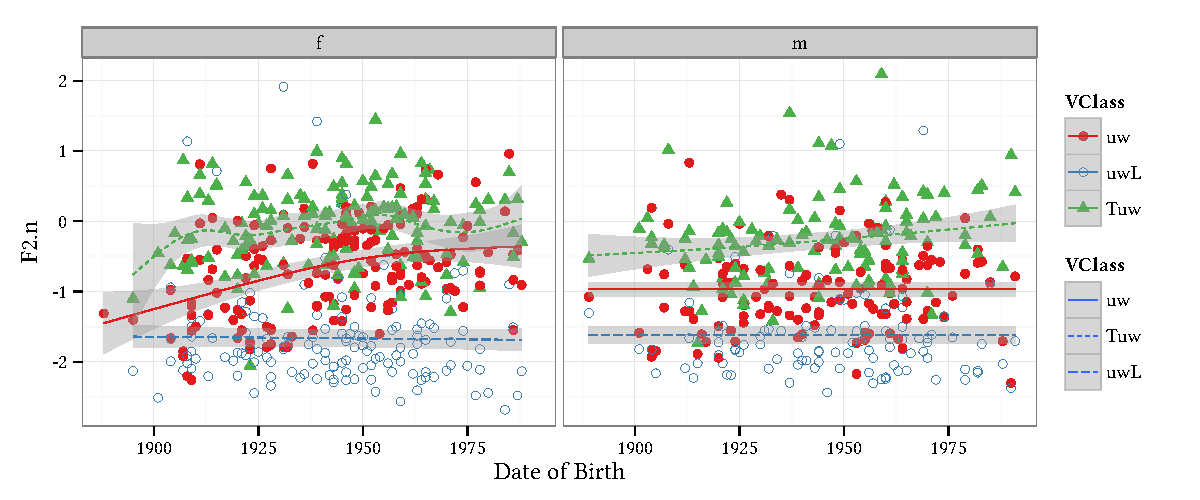
\includegraphics[width=1.13\textwidth]{figures/ch4uwBasicComp.pdf}
		\begin{center}
		
	\end{center}
\end{frame}

\begin{frame}{Sex and Change from Below, \textsl{um} \small{(Fruehwald, 2015, \textsl{inter alia}.) }\\ \small{n_{speakers} = 308, n_{tokens} = 25514}
%\begin{center}
		}
		
%	\end{center}
		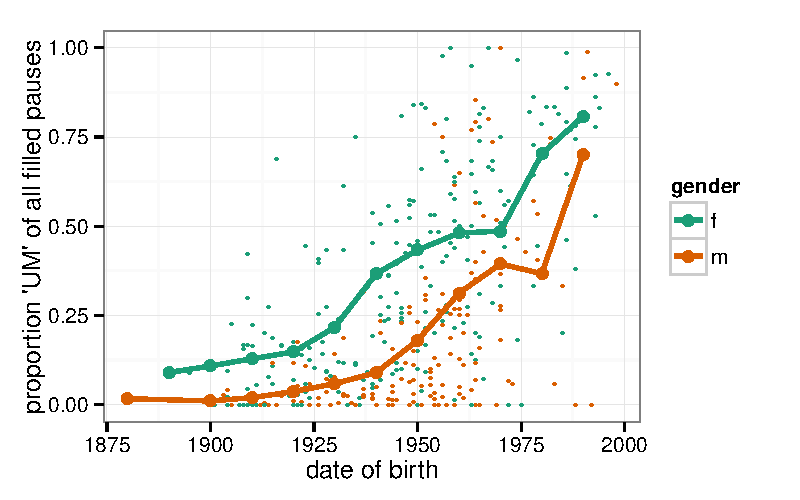
\includegraphics[width=1.12\textwidth]{figures/um.png}
	
	
\end{frame}



\subsection{Theories Proposed (and not proposed)}

\begin{frame}{\citet{labov2001}}
	\begin{enumerate}
		\item New variant initially spreads among women, by chance.
		\item All children get most of their linguistic input from women caregivers.
		\item Men in pre-adolescence retreat from women-led changes, so as to distinguish themselves socially.
		\item The change increments in each generation (reason unknown), with men staying behind women (and still retreating??).
	\end{enumerate}
%	\begin{center}
%		Labov entertains two possible biological possibilities, but dismisses them: one based on sexually dimorphic verbal ability, and another which only applies to vowels.
%	\end{center}
\end{frame}


\begin{frame}{\citet{eckert2011}}
	\begin{enumerate}
	\item New variant spreads anywhere in the population.
	\item In pre-adolescence, women figure out which is the new variant.
	\item Women adopt more of the new variant to distinguish themselves as ``trendy'' in the ``heterosexual marketplace''.
	\item Change increments in each generation because women continue this bias; implies people have implicit knowledge of the age-vector for a change \citep[weak evidence from][]{drager2011}.
	\end{enumerate}
\end{frame}

\begin{frame}{Problems with Labov, Eckert}
	\begin{itemize}
	\item Even though there's a proposed psychological and/or social effect, the mechanism for it is unexplained.
		\begin{itemize}
		\item Labov implicates men in retreating (something else pushes change forward).
		\item Eckert implicates women in pushing change forward (but something else must have spread it initially).
		\end{itemize}
	\item Also, one might question any social-signaling explanation: \textsl{um,uh} has lower mutual information for signaling sex than first or last letter of one's first name \citep{fruehwald2015}.
	\item Perhaps we can get closer to an explanation for some such effect, and while keeping in mind that speakers are unaware of these changes, and may not experience gender in a binary way.
	\end{itemize}
\end{frame}



%\begin{frame}{Blind Social Network (Bloomfield)}
%	\begin{enumerate}
%	\item Change spreads in women first, by chance.
%	\item Men jump on board at the same rate, and they never catch up.
%	\item The change increments in each generation for unknown reasons.
%	\end{enumerate}
%	\begin{itemize}
%	\item Possible problem with acquisition, from caregiver data \citep{smithetal2007}.
%	\item Must assume that there is no real trend for women to lead change from below.
%	\item Prediction: men should be 1 generation behind or less (?), with the lag remaining constant.
%	\end{itemize}
%\end{frame}



%chambers

\section{A biosocial model}

\begin{frame}{A biosocial model}
	\begin{itemize}
	\item[ ] \textbf{Theory:} pre-natal androgens affect how people learn socially, possibly mediated by gender identity.
	\end{itemize}

\end{frame}


%especially true in societies where women present much of the initial linguistic data to children
%incrementing change during adolescence
%julie-roberts showing kids probability match parents, DEJ work, child as linguistic historian


\subsection{Organising Effects on Behaviour}

\begin{frame}{Hormonal Organising Effects on Gender}
\begin{itemize}
	\item \citet{hinesetal2004}: Congenital Adrenal Hyperplasia (CAH) in XX, AFAB individuals has a significant effect on both \textbf{sexuality} and less female-typical/identifying \textbf{gender identity} both in childhood and adulthood, compared to controls.
	\begin{itemize}
	\item Also male/female-stereotypical \textbf{toy preference}, in \citet{pasterskietal2005}.
	\end{itemize}
	\item \citet{berenbaumbailey2003}: CAH was a significant predictor of \textbf{gender identity} in XX, AFAB individuals aged 18 and younger. (Interestingly, genital appearance was not, even when partly masculinized.)

\end{itemize}
\end{frame}

\begin{frame}{Hormonal Organising Effects on Gender}
\begin{itemize}

	\item \citet{hinesetal2002}: In a non-clinical population (ALSPAC \citealt{alspac2001}), found significant effect of maternal testosterone on childhood \textbf{gender-role behaviour} in XX, AFAB individuals aged 3.5, as assessed by the Pre-School Activities Index.
	\item \citet{auyeungetal2009} confirmed \citet{hinesetal2002}'s results predicting PSAI with amniotic fluid samples, gestation weeks 11-21, sample of 112 male, 100 female.
	\item Many other human and animal studied have found relationships between perinatal T and gendered behaviour or sexuality \citep[see][for reviews]{cohenbendahanetal2005, hines2006, balthazart2011, hinesetal2015}.
\end{itemize}
\end{frame}

\begin{frame}{Social Learning}
\begin{itemize}
	\item There are lots of non-human studies showing the result of hormonal organising on \textbf{brain morphology} \citep[e.g. in rats, going back to][]{gorski1978}, \textbf{sexuality} \citep[many references in][Chapts. 3-4]{balthazart2011}, and \textbf{birdsong} \citep[see][for an overview]{balthazartetal2009}.
	\item There's less explicitly on the effect of hormonal organising on social learning, though:
		\begin{itemize}
		\item This may be implicit in some of the human studies above
		\item May be implicit in the birdsong literature (though these do not always distinguish learning from production; see \citealt{balthazartetal2009}).
		\end{itemize}
	\item \citet{mansukhanietal1996}: zebra finch \textbf{pair-bonding}...
%		\begin{itemize}
%		\item hormone treatment (synthetic estradiol) significantly affected pair-bonding behaviours in colony tests \textbf{with females also raised in all-female aviaries}.
%		\item \textbf{Interpretation:} the masculinizing, organising changes due to affected the process of learning suitable models for pairing.
%		\end{itemize}

\end{itemize}

\end{frame}

\begin{frame}{\citet{mansukhanietal1996}}
\begin{block}{Results}
\begin{center}
	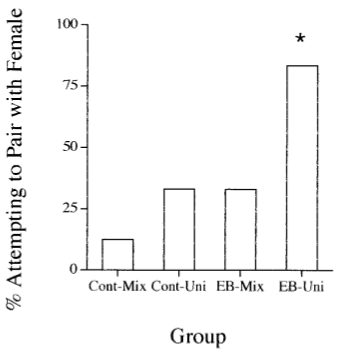
\includegraphics[width=.7\textwidth]{figures/gaybirds.png}
	\end{center}
\end{block}
\end{frame}

\begin{frame}{Social Learning}
\begin{itemize}

	\item Social behaviour: higher amniotic T predicts lower levels of \textbf{eye-contact} with caregivers/adults \citep{lutchmayaetal2002}
	\item \citet{knickmeyeretal2005}: significant relationship between amniotic T and scores on the ``Children's Communication Checklist'' in \textbf{pragmatic language use} and \textbf{social relationships} (58 children aged 4--4.25).
	\item Some unpublished experimental evidence suggests (Balthazart p.c., citing \citealt{hines2012}):
		\begin{itemize}
			\item Non-CAH women tend to mimic female models in an \textbf{artificial social learning task}.
			\item (non-CAH) men are not significantly affected by any models in the same task.
			\item CAH women are similarly unaffected, and not distinguishable from male participants.
		\end{itemize}
	\item Maybe linguistic studies will really fill a gap in the literature.
\end{itemize}

\end{frame}

\begin{frame}{A biosocial model}
	\begin{itemize}
	\item[ ] \textbf{Theory:} pre-natal androgens affect how people learn socially, possibly mediated by gender identity.
	\end{itemize}
	\begin{enumerate}
	\item New linguistic variant spreads anywhere first, by chance, driven by an unknown advantage (?).
	\item As speakers acquire it, they sample the whole population.
	\item Less T exposure leads to greater sensitivity to social models closer in age (and other respects).
	\item More T leads to less sensitivity to similar social models, sampling the population mean.
	\item More T speakers lag behind less T speakers.
	\end{enumerate}

\end{frame}

\begin{frame}{A biosocial model}
	\begin{itemize}
	\item \textbf{Hypothesis:} the difference should show up not only between different sex (genetic, genital, or assigned-at-birth) cohorts, but also within them by gradient or continuous gender.
	\end{itemize}
\end{frame}


\section{Pilot 1}


\begin{frame}{Sample}
\begin{itemize}
	\item 14 participants, all native speakers of English from Tyneside (4 participants overlap with Pilot 2).
	\item All assigned-female-at-birth (AFAB) and self-identifying as female.
	\item None have known endocrine disorders, or know their families to have endocrine conditions.
	\item Similar educational backgrounds: all attended secondary school, all some university
	\item Ages between 20-30 years old.
\end{itemize}
\end{frame}

\begin{frame}{Methodology}
\begin{itemize}
	\item Standard sociolinguistic interview procedures \citep{tagliamonte2006}; about an hour of speech per participant (interviewers Claire, Joel, and Annie Karatzenis), recorded digitally on Zoom H1 or H4n in wav.
		\begin{itemize}
			\item Basic personal and social history, including social network size (not analyzed yet).
			\item Module on sexuality and sexual history (not used at this point).
			\item Module on gender identity (not used at this point).
		\end{itemize}
	\item \textsl{um, uh} automatically extracted from transcripts, plus some phonological environment information.
	\item 2D:4D digit ratio:
		\begin{itemize}
		\item Annie's 10 participants by hand-tracings
		\item  4 with photocopies of right hands, 2D, 4D measured with Vernier digital calipers (Joel); \citet{allawayetal2009} found this to be the second most reliable method.
		\end{itemize}
\end{itemize}
\end{frame}


\begin{frame}{2D:4D ratio as proxy for pre-natal T}
\begin{itemize}
	%\item Broadly speaking, female ratios closer to 1, on average around 0.973, and male ratios smaller, average: 0.955 \citep[][107]{balthazart2011}.
	
	\item Sexual orientation: see extensive references in \citet{balthazart2011}, as well as rat models.
	\item 2D/4D difference in ``butch'' vs. ``femme'' self-report (gender?) in self-identified lesbians, with ``femme'' non-distinct from straight controls, but ``butch'' more masculinized \citep{brownetal2002}
	\item Experimentally manipulated in Wistar rats: maternal testosterone manipulation and direct pre-natal manipulation results in lower 2D/4D ratios in female rats, and also behavioral similarities to male rats in open field motor activity.\citep{talarovicovaetal2009}.
	\end{itemize}

\end{frame}

\begin{frame}{2D:4D ratio as proxy for pre-natal T}
\begin{itemize}
	%\item Broadly speaking, female ratios closer to 1, on average around 0.973, and male ratios smaller, average: 0.955 \citep[][107]{balthazart2011}.
	\item \citet{lutchmayaetal2004} found 2D:4D ratio reflected amniotic T/E ratio in 33 two-year-olds in \textbf{right hands}, using photocopies.
	\item (Note: effects are consistently more pronounced on right hands in both humans and rodents, as in \citealt{brownetal2002} and \citealt{talarovicovaetal2009}; see also review in \citealt{cohenbendahanetal2005}).
\end{itemize}

\end{frame}


\begin{frame}{2D:4D ratio: smaller $\rightarrow$ more pre-natal T (or T/E)}
\begin{center}
	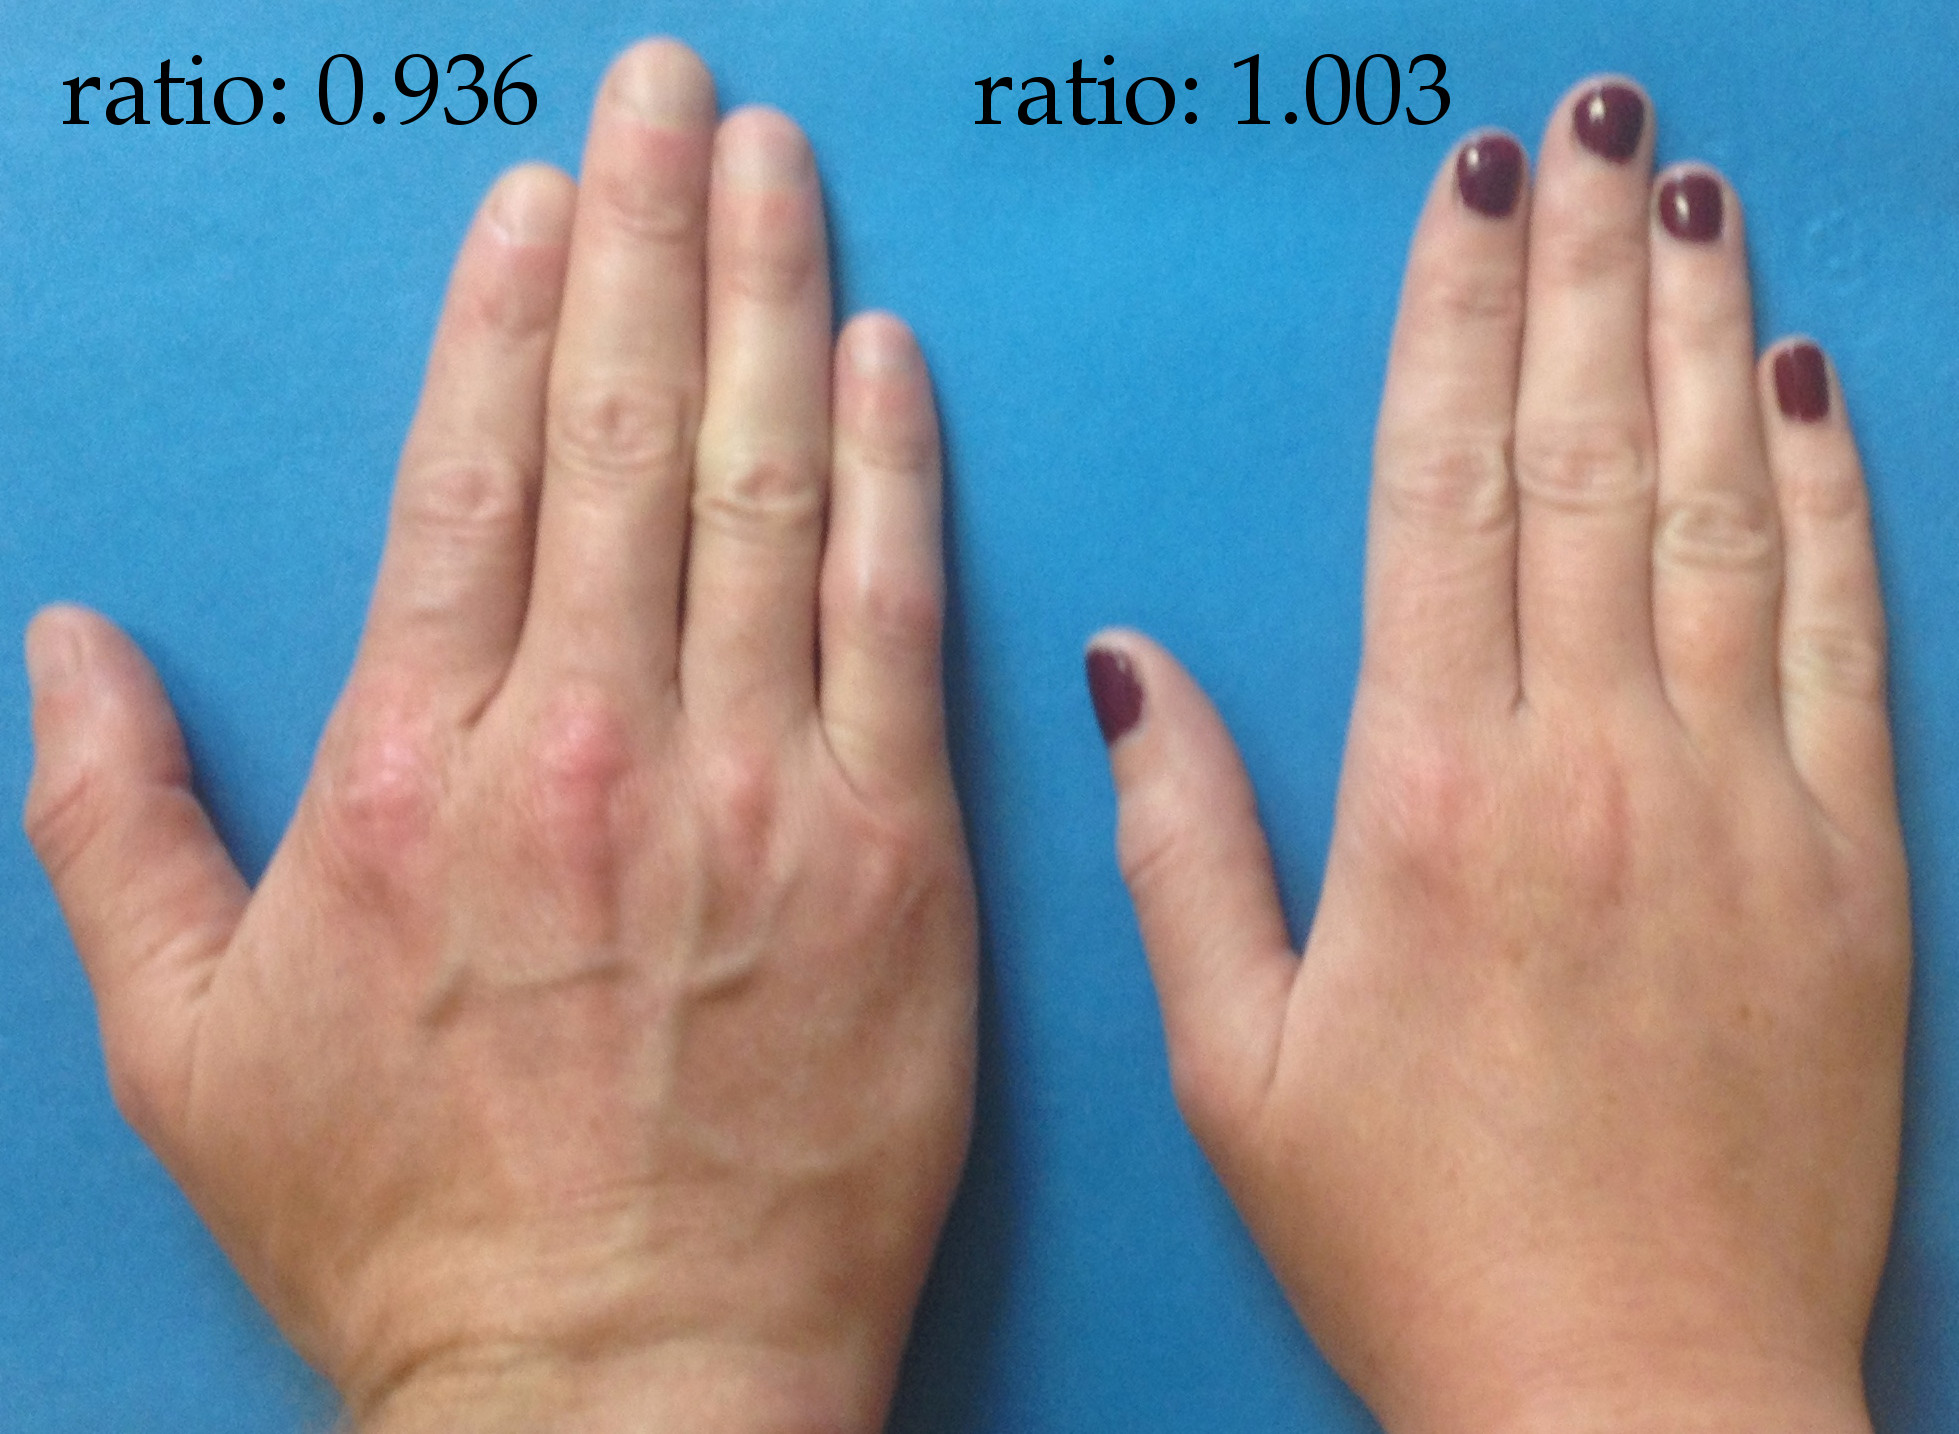
\includegraphics[width=1.12\textwidth]{figures/realhands2.jpg}
\end{center}
\end{frame}


\begin{frame}{Results of Pilot 1}
%\begin{center}
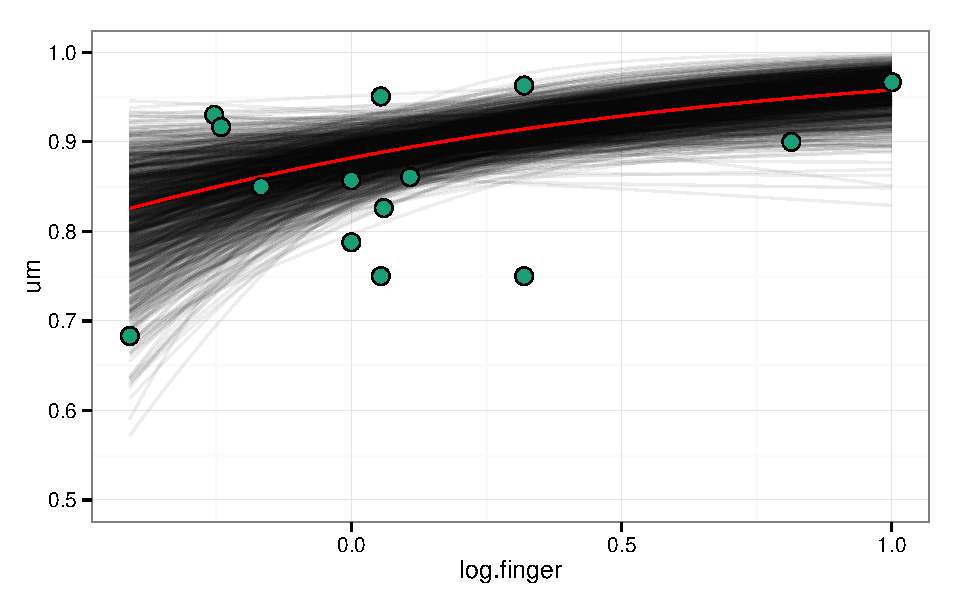
\includegraphics[width=1.12\textwidth]{figures/fingereffect.pdf}
%\end{center}
\end{frame}


\begin{frame}{Results of Pilot 1}
\begin{itemize}
\item 1,000 bootstrap replicates produce a CI that excludes 0: (0.095,  2.567), and a permutation test (10,000 permutations) yields $p$ = 0.0563. Model fit of a mixed effects logistic regression on log(digit\_ratio):
\end{itemize}
\begin{center}
\begin{tabular}{rrrr}
\toprule
	model & AIC & BIC & LR p-value\\
	\cmidrule{2-4}
without ratio & 813.14 & 842.64 & -- \\
with ratio &  811.36 & 845.79 & 0.052\\
\bottomrule
\end{tabular}
\end{center}

\end{frame}


\begin{frame}{Results of Pilot 1}
\noindent Effect size in a mixed effects logistic regression on log(digit\_ratio): the same order of magnitude as female effect on \textsl{um,uh} in other spoken corpora (Wieling et al, \textsl{forthcoming}).
\begin{center}
\begin{tabular}{l r}
\toprule
\textbf{Sample} & \textbf{Effect Size}\\
\midrule
Female effect, HCRC Maptask & 2.3\\
Female effect,Fischer Corpus & 1.37\\
Female effect, PNC & 1.31\\
\textbf{Finger Ratio, our Pilot 1} & \textbf{1.12}\\
Female effect, Switchboard Corpus & 1.03\\
Female effect, British National Corpus & 0.45\\
\bottomrule
\end{tabular}
\end{center}

\end{frame}


\section{Pilot 2}


\begin{frame}{Sample}
\begin{itemize}
	\item 17 participants, all native speakers of English from Tyneside (4 overlap with Pilot 1).
	\item All assigned-female-at-birth (AFAB) and self-identifying as female.
	\item None have known endocrine disorders, or know their families to have endocrine conditions.
	\item Similar educational backgrounds: all attended secondary school, nearly all some university.
	\item Ages between 20-45 years old.
\end{itemize}
\end{frame}

\begin{frame}{Methodology}
\begin{itemize}
	\item Standard sociolinguistic interview; > an hour of speech per participant (interviewers Claire and Joel), recorded digitally on Zoom H4n in wav.
		\begin{itemize}
			\item Basic personal and social history, including social network size (not analyzed yet).
			%\item Asked whether or not they were called ``tomboy''
			\item Module on sexuality and sexual history, coded later in Kinsey scores (0-6) by Joel
			\item Module on gender identity.
			\item Transcribed (Claire, Caitlin, Charlotte).
		\end{itemize}
	\item \textsl{um, uh} automatically extracted from transcripts, plus some phonological environment information.
	\item 2D:4D digit ratio: photocopies of right hands, 2D, 4D measured with Vernier digital calipers (Joel).
	\item Gender scale task, also measured with digital calipers, converted to ratio.
\end{itemize}
\end{frame}

\begin{frame}{Gender Scale}
\begin{center}
	\includegraphics[width=1.12\textwidth]{figures/scale.png}
\end{center}
\end{frame}




\begin{frame}{Results of Pilot 2 (excluding an outlier)}
\begin{itemize}
\item A permutation test (10,000 permutations) yields $p$ = 0.26, CI includes 0. Model fit of a mixed effects logistic regression on log(digit\_ratio):
\end{itemize}
\begin{center}
\begin{tabular}{rrrr}
\toprule
	model & AIC & BIC & LR p-value\\
	\cmidrule{2-4}
without ratio & 1484.0 & 1518.1 & -- \\
with ratio &  1483.6 & 1512.1 & 0.1997\\
\bottomrule
\end{tabular}
\end{center}

\end{frame}

\begin{frame}{Results of Pilot 2: Digit Ratio vs. \textsl{um,uh}}
%\begin{center}
\includegraphics[width=1.12\textwidth]{figures/digitum2.pdf}
%\end{center}
\end{frame}

\begin{frame}{Results of Pilot 2: Digit Ratio vs. Gender Scale}
%\begin{center}
\includegraphics[width=1.12\textwidth]{figures/digitgender.pdf}
%\end{center}
\end{frame}


\begin{frame}{Results of Pilot 2}
\noindent Effect size in a mixed effects logistic regression: as large or larger than female effect in other spoken corpora, but with less confidence.\begin{center}
\begin{tabular}{l r}
\toprule
\textbf{Sample} & \textbf{Effect Size}\\
\midrule
\textbf{Digit Ratio, our Pilot 2} & \textbf{2.44}\\
Female effect, HCRC Maptask & 2.3\\
Female effect,Fischer Corpus & 1.37\\
Female effect, PNC & 1.31\\
\textbf{Digit Ratio, our Pilot 1} & \textbf{1.12}\\
Female effect, Switchboard Corpus & 1.03\\
Female effect, British National Corpus & 0.45\\
\bottomrule
\end{tabular}
\end{center}

\end{frame}


\begin{frame}{Things to think about...}
\begin{itemize}
	\item Luck of the draw with a small sample size? We need a larger sample. (And there's an outlier...)
	\item Digit ratios are variable, measurements are noisy, and we should move to scans.
	\item Better linguistic variable? Maybe \textsl{um, uh} change is too close to done.
	\item Increased age range to increase variability, but creates modeling challenges in a small dataset.
	\item How do we deal with correlated effects of gender, sexuality?
\end{itemize}
\end{frame}


\begin{frame}{Results of Pilot 2: Age vs. \textsl{um,uh} (with Jay)}
%\begin{center}
\includegraphics[width=1.12\textwidth]{figures/ageumJay.pdf}
%\end{center}
\end{frame}


\begin{frame}{Results of Pilot 2: Age vs. \textsl{um,uh} (without Jay)}
%\begin{center}
\includegraphics[width=1.12\textwidth]{figures/ageum.pdf}
%\end{center}
\end{frame}


\section{Our (Future) Study}

\begin{frame}{Future Study}
\begin{itemize}
	\item A sample of 200 participants from ALSPAC
	\item Assays for maternal T and estradiol. (To the extent possible, we will sample the same participants studied in \citealt{hinesetal2002}). 
	\item Standard sociolinguistic interview procedures.
	\item Semi-automatic extraction of changes in progress from transcribed audio.
	\item 2D:4D from scans using virtual calipers in pixels, sexuality info, gender info, using whichever self-report mechanisms seem to be most reliable.
\end{itemize}
\end{frame}


\begin{frame}{Future Study: Hypothesis}

\begin{center}
\item If linguistic variables are learnt differentially depending on how masculinised brain structures have been by pre-natal androgen levels, then:
\end{center} 
\begin{itemize}
	\item Within a given sex cohort (i.e. genital-sex, or sex designated at birth), more advanced linguistic variants correspond to lower levels of pre-natal T, and perhaps other androgens (esp. women).
	\item If the gender effect in language is purely social, then we should see no effect of hormones within each sex (only between sexes).
\end{itemize}
\end{frame}


%\begin{frame}{butch femme?}
%\begin{itemize}
%	\item stuff
%	\end{itemize}

%\end{frame}


\section{Conclusions}


\begin{frame}{Conclusions}
%	\begin{block}{Conclusions}
		\begin{itemize}
			\item There's no consensus on reported linguistic sex effects, though there are a few ideas.
			\item Hormonal organising effects suggests a partly biological, partly social model, with the following properties:
		\begin{itemize}
			\item It could explain both sex/gender effects based on independently attested mechanisms.
			\item The view of gender is interestingly non-binary or gradient, which tallies with people's self-reports of gender identity.
			\end{itemize}
			%\item Though we'd like more independent data on social learning, this study could provide additional evidence.
			\item Linguistic productions could be a more precise measure of social learning, than rougher questionnaire and experimental techniques.
			\item Question: how much does this have to do with gender, after all?
	\end{itemize}
%	\end{block}
\end{frame}




\begin{frame}{Acknowledgements}
\begin{center}

Special thanks to Jacques Balthazart, for being highly available; to our past student Anne-Marie Karatzenis; To Daniel Nettle, Tom Smulders, and Bonnie Auyeung for discussion. To our RAs Claire Cochrane, Caitlin Halfacre, Charlotte Huggins.

A number of individuals in the Newcastle transgender community have graciously given their input into how we ask for gender self-reports.

%\vspace{5mm}\\
%Simulation: \texttt{github.com/joelcw/tyneside/blob/master/articles/sim\_Gauss.R}
%\vspace{1mm}\\
%Extraposition Study: \texttt{github.com/joelcw/tyneside/tree/master/extraposition}
\end{center}
\end{frame}



\begin{frame}[allowframebreaks]
\frametitle{References}
\newcommand*{\newblock}{natbib}
\bibliographystyle{linquiry2}
\bibliography{joelrefs}
\end{frame}

\begin{frame}{The socio-biological model \\\small{(Version 2; based on Kevin Stadler's work)}}
	\begin{itemize}
	\item \textbf{Theory:} one effect of hormonal organising effects is on how people learn socially from models of different sex/gender.
	\item Learning from social models differs by gender (and so is roughly sexually dimorphic).
	\end{itemize}
	\begin{enumerate}
	\item Women copy women more than men copy anyone.
	\item The change arises because women sampling finite utterances from women perceive a change.
	\item There's systematic overshoot in women's productions as they try to copy, in the direction of a perceived trend, which drives the change.
	\item Men should be about one generation behind (?).
	\end{enumerate}

\end{frame}



\begin{frame}{\citet{mansukhanietal1996}}
\begin{block}{Study Design}
\begin{itemize}
	\item Pair-bonding preferences in female zebra-finches, who partner for life.
	\item Not the same as mating-preferences, which have been investigated in a number of species; presumably more related to social learning.
	\item 30 females, in two conditions: raised in all-female aviaries vs. mixed aviaries, and treatment with estradiol benzoate (synthetic estradiol) vs. no treatment
		\begin{itemize}
		\item All subsequently given hormone treatments to equalize adult circulating hormone levels.
		\end{itemize}
\end{itemize}
\end{block}
\end{frame}

\begin{frame}{\citet{mansukhanietal1996}}
\begin{block}{Results}
\begin{itemize}
	\item Significant effects of EB treatment on plumage, singing, dancing, and mounting behaviours in choice tests.
	\item However, EB treatment only significantly affected pair-bonding behaviours in colony tests \textbf{with females also raised in all-female aviaries}.
	\item \textbf{Interpretation:} the masculinizing, organisational effect of estradiol affected the process of learning suitable models for pairing.
	\item The brain structures affected must be implicated in social learning, beyond directly instinctual behaviours (e.g. mounting, dancing (?))
		\begin{itemize}
			\item The singing data is ambiguous, since it must be learned, but we don't know which part of the song system has been changed here \citep[see][]{balthazartetal2009}.
		\end{itemize}
	\end{itemize}
\end{block}
\end{frame}



\end{document}